\documentclass[a4paper,11pt]{article}
\usepackage[margin=1in]{geometry}
%%%\usepackage[utf8]{inputenc}
\usepackage{pslatex}


\usepackage{comment}

\usepackage{graphicx}
\usepackage[]{parskip}

\usepackage{listings}
\usepackage{color}
 
\definecolor{codegreen}{rgb}{0,0.6,0}
\definecolor{codegray}{rgb}{0.5,0.5,0.5}
\definecolor{codepurple}{rgb}{0.58,0,0.82}
\definecolor{backcolour}{rgb}{0.95,0.95,0.92}
 
\lstdefinestyle{etdportal}{
    backgroundcolor=\color{backcolour},   
    commentstyle=\color{codegreen},
    keywordstyle=\color{magenta},
    frame=single,
    numberstyle=\tiny\color{codegray},
    stringstyle=\color{codepurple},
    basicstyle=\footnotesize,
    breakatwhitespace=false,         
    breaklines=true,                 
    captionpos=b,                    
    keepspaces=true,                 
    numbers=none,                    
    numbersep=5pt,                  
    showspaces=false,                
    showstringspaces=false,
    showtabs=false,                  
    tabsize=2
}

\lstset{style=etdportal}

\usepackage[ps2pdf,bookmarks=true]{hyperref}
\hypersetup{pdftitle={Electronic Thesis and Dissertation Portal Manual},pdfauthor={Lawrence Webley, Lighton Phiri, Hussein Suleman}, pdfsubject={Repository Software}, pdfkeywords={Digital Libraries, ETDPortal, NRF, OAI-PMH, Repository}, pdfview={FitH},pdfstartview={Fit}}

\hypersetup{colorlinks,linkcolor=blue,citecolor=blue,urlcolor=blue,bookmarksnumbered}

% This needs to be after hyperref
\usepackage{cleveref}

%opening
\title{Electronic Thesis and Dissertation Portal Manual\\Version 1.2}
\author{
Authors\\
Lawrence Webley\\
\textless \href{mailto:lwebley@cs.uct.ac.za}{lwebley@cs.uct.ac.za} \textgreater \\
Lighton Phiri\\
\textless \href{mailto:lphiri@cs.uct.ac.za}{lphiri@cs.uct.ac.za} \textgreater \\
Hussein Suleman\\ 
\textless \href{mailto:hussein@cs.uct.ac.za}{hussein@cs.uct.ac.za} \textgreater \\
}
\date
{
September 2016
}

\begin{document}

\maketitle
\thispagestyle{empty}
\newpage
\tableofcontents
\thispagestyle{empty}
\newpage

\section{General overview}

The ETD (Electronic Thesis and Dissertations) repository and portal software is composed of three distinct components, each of which operates fairly independently of the other. The three sections are:

\subsection{Harvester module}

This program is run by the system at regular intervals and serves to download thesis records from institutions and then store them in the local database. The entire thesis is not downloaded, simply the metadata, including the thesis name, the author and a short summary of the paper. These records are stored in an XML format (usually OAI\_DC or OAI\_MARC). The servers that this program harvests from are known as repositories and are located at academic. These repositories provide access to their records via the OAI-PMH protocol, and the harvester uses this protocol to harvest all new records on the remote server (i.e. the harvester does not fetch the entire database each time, only records that have changed or been added).

When the harvester runs it will sequentially go through each of the repositories that it knows about and attempt to harvest from each. Each repository it harvests from has its own configuration record that will also store the harvest status of the repository (when it was last harvested, if a harvest is currently in progress or if an error has occurred during the last harvest).

Another section of the harvester is the Harvester Control Panel. This is accessed via the front Web page (the Web portal) and is used to administer and manage the list of repositories. The control panel can be used to add, modify and delete repositories as well as initiate an immediate harvest on any of the available repositories. It also allows an administrator to see the current progress of a given harvest and see the results of past harvests.

\subsection{Local repository module}

The second major part of the project is the local repository. All the records that have been harvested by the harvester component are stored in a local MySQL database, which is not accessible directly from the outside. The repository component provides an OAI-PMH read-only interface through which other servers can access the local database. The repository accepts Web requests and replies using XML pages, which conform to the OAI-PMH 2.0 standard. This means that any remote institution that would like to download or access the database can use this repository to do it programmatically. The harvester and the repository share a common SQL database and common tables.

The repository is also how the front end Web component of the program access the records stored in the database and as such the front end Web page segment could easily be hosted on a different server to the repository and harvester.

Another smaller part of the repository is the RSS and Summary software. This small program will provide a RSS feed to interested users, listing the latest records to be added to the server and will provide statistics detailing the number of records stored in the system, and from which institution they come.

\subsection{Web portal module}

The third, most visible, component of the project is the Web Portal. This is what online users see when they access the ETD site. It uses the Lucene\footnote{http://lucene.apache.org} open source search engine to search through records. The front end portal uses the local repository to access the harvested records. It has its own tables in a MySQL database, which it uses to index the records it reads from the repository. These are the tables it uses to process search queries from the Web.

\section{File layout}

After installation all configuration files will reside in \path{/etc/etdportal}. All the application files will be in \path{/var/lib/tomcat7/webapps}. Lucenes' index files are stored in \path{/var/db/index}. Each servlet has its own folder within webapps, named after the servlet. Each of these folders will contain a \texttt{WEB-INF} folder, which is recognised by tomcat. Inside the \texttt{WEB-INF} folders of each servlet will be at least two more folders: \texttt{classes} and \texttt{lib}. The classes folder contains the java class files, which contain all the code for the servlets. The lib folders contain libraries necessary for the servlets to function. The \texttt{web.xml} file located in the \texttt{WEB-INF} directory of each servlet contains the path that each servlet will have when accessed via URL.

\section{Database layout}

There are two separate databases used for the harvester and repository backend and the Web portal front end.

\subsection{Harvester and repository database}

All records in the database are stored in a table named Archive which contains all the harvested records. The records in this database are inserted by the harvester and read by the OAI-PMH repository software. The fields contained are: ID (the record identifier), Date (the date the record was harvested), MetaType (the xml format record), Source (the URL of the repository this record was harvested from), Deleted (whether or not this record has been deleted - the records are never totally deleted; they are simply marked as such for synchronisation issues), About (any additional data about the record that was retrieved) and SetSpec (the repository set that this record belongs to).
The primary key of the table is a combination of the ID and the MetaType fields. This means that there can be multiple records with the same ID, as long as their metadata formats are not the same (same record in a different format).
The second table is named Repositories and contains a list of the repositories that can be harvested. This list is controlled through the harvester control panel. The fields in this table are: ID (Repository set name), name (repository human readable name), isRunning (determines whether a harvest is currently running on a given repository), harvestStatus (details the last harvest run, or the progress of a current one), baseURL (the URL of the remote service we would like to harvest from), metadataFormat (the format we would like to harvest from the remote server), setSpec ( the short (no spaces) name that will be used as the set identifier for the target repository), dateFrom ( the last time this repository was harvested) and harvestInterval (the minimum time in seconds between harvest attempts on the repository).

\subsection{Web portal database}

The portal database contains a collection of interlinked tables which are used to efficiently browse through the records by category. The tables are named descriptively and thus the purpose of most is self evident. These tables are automatically generated by the portal's indexer and should not be manually edited.

\section{Installation process}

The following instructions assume that the server will be running Ubuntu---testing has been done on Ubuntu 10.04 and 16.04. If you are running a different operating system, please adapt them accordingly.

\subsection{Pre-requisites}

Before installing the ETD software, a few prerequisite programs need to be installed. If any of the below programs are not installed, follow the steps below to install them. Firstly the Java JDK must be available. To install Java type the following into an open console window: 

\begin{lstlisting}[language=bash]
 sudo apt-get install openjdk-8-jdk
\end{lstlisting}


Follow the prompts to finish installing Java. Next you must ensure that Tomcat6 is installed. To install tomcat, type the following into an open console window: 

\begin{lstlisting}[language=bash]
 sudo apt-get install tomcat7
\end{lstlisting}


Again follow the prompts to complete installation. You must also have an Apache Web server available. To install the Apache Web server type the following into a open console window: 

\begin{lstlisting}[language=bash]
 sudo apt-get install apache2
\end{lstlisting}

And follow the prompts to install it. This should complete the installation of the prerequisite software, and you should now be able to go on to the main installation. We also need MySQL installed for the program databases (if it is not already installed): 

\begin{lstlisting}[language=bash]
 sudo apt-get install mysql-server
\end{lstlisting}

\subsection{Installation}

Currently we are using the GIT version control system to work on the software. To get the latest version, browse to a folder where you would like to put the installation files and type the following:

\begin{lstlisting}[language=bash]
git clone git@simba.cs.uct.ac.za:etdportal.git 
git checkout v1.2
\end{lstlisting}

Once you have the software available, open a console window and navigate to the folder containing the ETD software. To compile the software (on a non read-only disk, such as a hard drive) type the following into the console window: 

\begin{lstlisting}[language=bash]
 make
\end{lstlisting}

This will compile the necessary files for use. Next type in the following to install the software in the correct locations: 

\begin{lstlisting}[language=bash]
 sudo make install
\end{lstlisting}

This will install the software into the correct locations. The make clean command is available to delete all compiled or auto-generated files in case you would like to recompile the project.

\subsection{Database setup}

Now we need to set up the MySQL databases that the server will use to store records. We will need two separate databases for the software---one for the harvester and repository and the other for the Web portal. Create two empty databases with different usernames and passwords. 

\begin{lstlisting}[language=SQL]
 CREATE USER 'etduser'@'localhost' IDENTIFIED BY 'etduser'; 
 CREATE DATABASE etd_dba; 
 CREATE DATABASE etd_dbb; 
GRANT ALL ON etd_dba.* TO 'etduser'@'localhost';
GRANT ALL ON etd_dba.* TO 'etduser'@'localhost';
\end{lstlisting}

We will use a SQL script to create the required tables: 

\begin{lstlisting}[language=bash]
 mysql etd_dba < harvester/WEB-INF/db/create_db.sql -u etduser -p
\end{lstlisting}

And do the same for the other database. 

\begin{lstlisting}[language=bash]
 mysql etd_dbb < portal/WEB-INF/db/create_db.sql -u etduser -p
\end{lstlisting}

Once this is done, you should have two separate databases: the repository database with 2 tables in it and the portal database with 12 tables in it. This concludes the database setup.

\subsection{Configuration files}

Now we need to configure the software for the local system. To start doing this we need to create a basic configuration file. Start by navigating to \path{/etc/etdportal/}.

Once there, copy the \texttt{config.xml.orig} to \texttt{config.xml} and customize the configuration file for the server. 

\begin{lstlisting}[language=bash]
 sudo cp config.xml.orig config.xml 
 sudo gedit config.xml
\end{lstlisting}

In the configuration file, remember to change the preset database details that are there to the ones you set in the database set up. Now we need to add a manager account to the tomcat users file so that we can access the harvester control panel securely. 

\begin{lstlisting}[language=bash]
 sudo gedit /var/lib/tomcat7/conf/tomcat-users.xml
\end{lstlisting}

Once open add a new role for netdmanager in the \textless tomcat-users\textgreater \, tag and add a new username and password with this role. 

\begin{lstlisting}[language=XML]
 <role rolename=netdmanager/> 
 <user username=mandy password=your\_pass roles=netdmanager/>
\end{lstlisting}

\subsection{Apache2}

The servlets will now function, but they will not be easy to access, so we need to make the portal servlet the first thing tomcat shows, and then we need to make tomcat the first thing apache shows.

Open \texttt{/var/lib/tomcat7/conf/server.xml} (as root) and add 

\begin{lstlisting}[language=XML]
 <Context path="" docBase=portal//> 
\end{lstlisting}

inside the \texttt{<Host>} tags (so just below the line with \texttt{xmlValidation=false xmlNameSpaceAware=false>})

Now we need to configure apache: 

\begin{lstlisting}[language=bash]
 a2enmod rewrite 
 a2enmod proxy 
 a2enmod proxy_http 
 a2ensite etd
\end{lstlisting}

And then we change the servername field to \texttt{www.netd.ac.za } in \path{/etc/apache2/sites-available/etd} (as root).

If we are testing on a local machine, we need to add www.netd.ac.za to the \path{/etc/hosts} file at the end of line starting with \texttt{127.0.0.1}.

Finally we need to restart the apache web server: 

\begin{lstlisting}[language=bash]
 /etc/init.d/apache2 restart
\end{lstlisting}

And restart the tomcat server: 

\begin{lstlisting}[language=bash]
 /etc/init.d/tomcat7 restart
\end{lstlisting}

\subsection{Crobtab}

Once the portal has been set up, we need to set up cron (linux scheduler) to regularly run the harvester program. The harvester program will automatically decide which repositories need to be harvested and do so accordingly, but it needs to be called regularly to do this. After the harvester finishes a harvest, the Web portal needs to be run to keep the index up to date. The easiest way to do this is using a shell script. The script is located at \path{/var/lib/tomcat7/webapps/Harvest.sh}

Adding the script to a cron job that runs every hour is done as follows: 

\begin{lstlisting}[language=bash]
 crontab -e
\end{lstlisting}

and then enter the following into the editor provided : 

\begin{lstlisting}[language=bash]
 0 * * * * /var/lib/tomcat7/webapps/Harvest.sh
\end{lstlisting}

This will cause cron to run the Harvest script every hour, on the hour.

\section{Using the control panel}

To access the control panel you must click on Admin on the bottom of the left side bar of the Web site. The username and password will be those that you set up during the Setting up the configuration files part of the installation. Once logged on you will be faced with a list of known repositories. To start with this will be empty. The status of a harvest can also be seen from this control panel home page under the status column. If a harvest has been completed recently, the number of harvested records will appear in the status column. If a harvest is currently in progress, the current number of records processed will show under the status column.

\subsection{Adding a repository}

\begin{figure}[h]
 \centering
 \fbox{%
   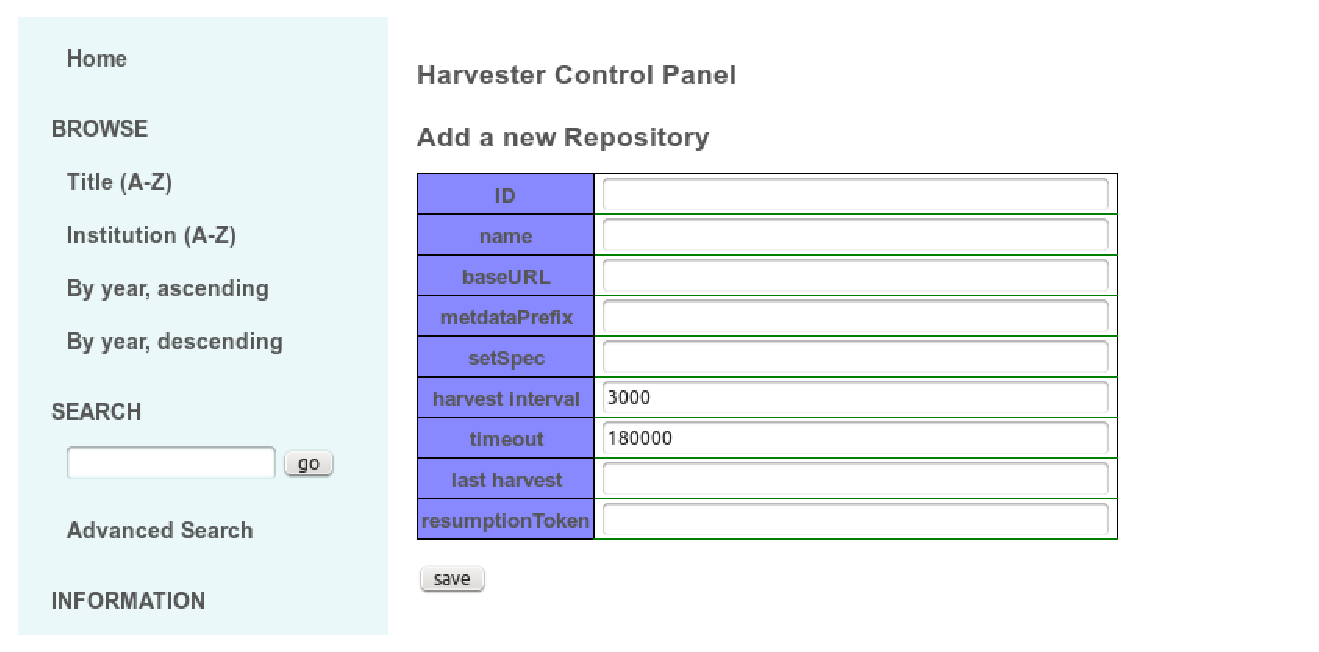
\includegraphics[width=\textwidth]{adding_repository_infomation_x.eps}%
 }%
 \caption{Adding a new repository entry}
 \label{adding_repository_information}
\end{figure}

To add a new repository for harvesting, click the Add Repository link at the bottom of the center window. The screenshot in \Cref{adding_repository_information} will appear. Here is a summary of what each of the fields below mean.
ID: The short (no spaces) name that is used to identify where records come from (can't change once set). Name: Full Institution name BaseURL: The url of the servlet that we wish to harvest from. Must include the http://. MetadataPrefix: The format of the metadata we wish to harvest. Some repositories will support multiple formats. SetSpec: The remote server's set that we wish to harvest. Leave this empty to harvest the whole repository. Harvest Interval: Time in seconds between consecutive harvests of this repository. Last Harvest: When to harvest from (will automatically be set to the last harvest date after each harvest). Delete this to perform a full re-harvest of a repository.
The required fields are ID, Name, BaseURL and metadataPrefix. Once these are filled in, you can press save to save the repository. At the next scheduled harvest, the harvester will perform a full harvest of this new repository.

\subsection{Editing a repository}

\begin{figure}[h]
 \centering
 \fbox{%
   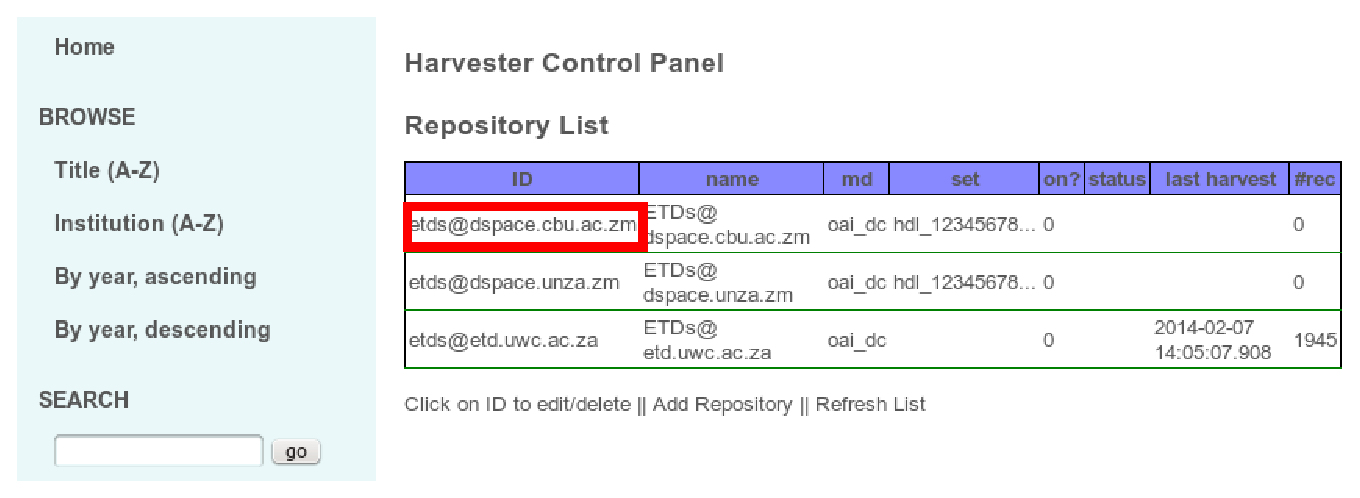
\includegraphics[width=\textwidth]{editing_repository_infomation_x-stroked.eps}%
 }%
 \caption{Editing repository entries information}
 \label{editing_repository_information}
\end{figure}

To edit a repository that is already there, simply click on the repository's ID tag in the repository list, as highlighted in \Cref{editing_repository_information}.
This will bring up the same form as for creating a new repository, except with the clicked-on repository's settings. Once done editing, remember to click save.

\subsection{Deleting a repository}

\begin{figure}[h]
 \centering
 \fbox{%
   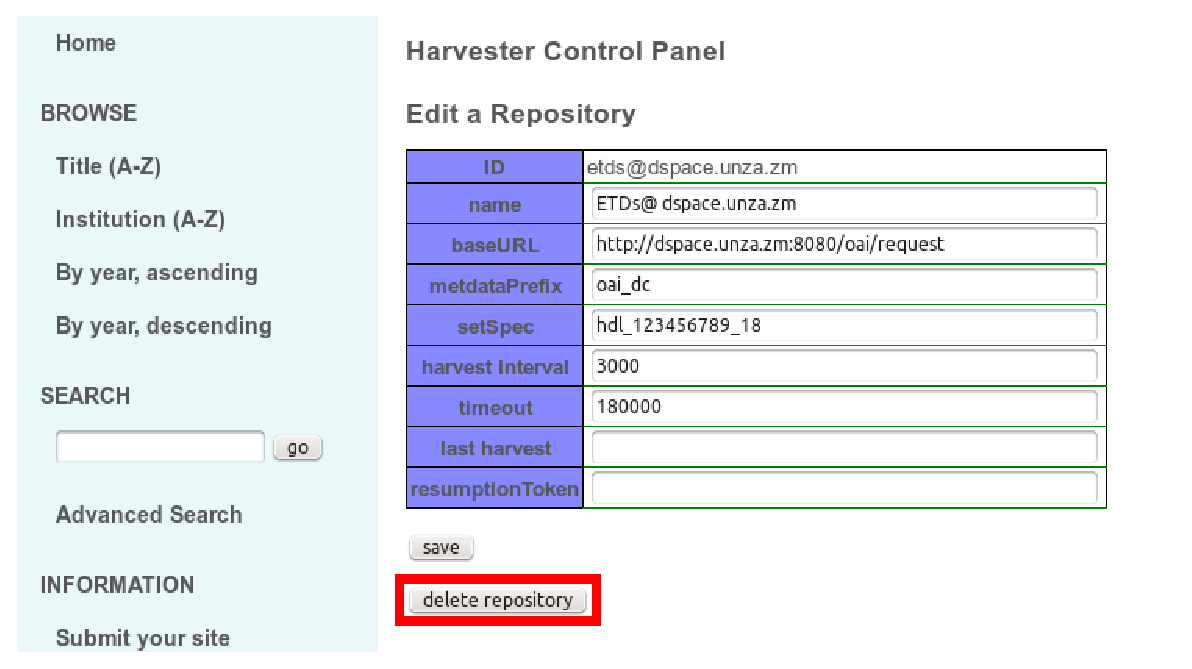
\includegraphics[width=\textwidth]{deleting_repository_infomation_x-stroked.eps}%
 }%
 \caption{Deleting existing repository entries}
 \label{deleting_repository_entry}
\end{figure}

To delete repository, click on the repository's ID, as above in Editing a repository, but instead of clicking save at the bottom of the screen, click delete repository, as shown in \Cref{deleting_repository_entry}.

\section{Class summaries}

\subsection{Harvester}

The harvester servlet is the part of the program that retrieves records from a remote repository and then stores them locally in an SQL database.

OAIHarvest: Is the entry point for the harvesting process. If passed no arguments it will check all repositories in the database to see if they need harvesting. If passed a repository ID, it will harvest that particular repository.

Config: Information for the database that has been read from the configuration files.

Database: A database interaction file that serves as an interface for the harvester to interact with the SQL database.

Repository: A class that loads and stores configuration details about a particular repository or harvest. This represents the state of a harvest and will update the repository information as the harvest progresses.

OAIRequest: A class to send a request and process a response from an OAI source.

OAIResponseHandler: Stores and parses the response to the OAI-PMH request in the database.

OAIRecord: Object to represent a single record.

HarvesterControlPanel: Responsible for constructing the harvester control panel and processing the actions associated with it.

HTMLWriter: A utility class used to wrap the harvester control panel output in valid html tags.

\subsection{Repository}

The repository provides a standardised interface for public entities to access the records database. All requests are via URL's and all replies are via XML output.

Config: Floating object containing configuration information for the server. Passed from class to class.

DatabaseConnection: Connects to the SQL database and is used to perform any database queries.

OAIServlet: Inherits from HttpServlet. This is the starting point for the repository program, and depending on the URL string received, a different action will be carried out.

Response: Abstract class providing a generic layout for a servlet response. Each verb will inherit from this class to provide its response.

ResponseFormatter: A utility class to write out the generic information at the beginning and end of an OAI-PMH XML file, inserting the different response content in the correct spots.

CheckParams: A utility class used to check whether the given URL parameters are in the correct format and are all expected. If they aren't, the servlet will provide an error response.

GetRecord: Inherits Response. Class to handle the GetRecord request.

Identify: Inherits Response. Class to deal with an Identify request.

ListIdentifiers: Inherits Response. Class to deal with a ListIdentifiers request.

ListMetadataFormats: Inherits Response. Lists the currently supported metadata formats of the server (based on config.xml).

ListRecords: Inherits Response. Lists all records that fall within the given parameters.

ListSets: Inherits Response. Lists all sets in the repository.

\subsection{Web portal}

The Web portal is what users see when they access the site from the outside. It is responsible for providing search and browse services, and thus must index the database records in a database of its own.

ConfigurationManager: Controls access to and sharing of configuration settings.

DatabaseBrowser: Used to run MySQL queries on the portal database.

DatabaseUpdater: Creates a link with the repository database and updates any new records that have been captured by the harvester into the portal database.

FileDocument: Creates Lucene Documents for indexing a metadata record.

HarvestingMain: Used to run the application that will harvest data from the local repository and place it in database tables that will make it easier for users to browse the data in the online application interface.

HarvestRequest: Contains all the OAI-PMH requests for the metadata harvester.

Index: Dynamically generates the index page.

IndexFiles: Used to index all the records that are within the repository database so that they can be searched easily.

Record: Represents an object formed from the xml record that is read from the repository.

ResponseParser: This class is used to parse the responses that are received from the server

ResultFormat: Formats the results that have been returned from a browsing request.

ResumptionToken: Forms an object that represents the resumption token returned by the repository in a list records request.

SearchEngine: This class is used to run a search query on the index created by the IndexFiles class using the Lucene library.

\appendix

\section{Installation package}

\begin{lstlisting}[language=bash]
phiri@phiri-PROLINE-DH55TC:~/Sandbox$ tree -d etdportal/
etdportal/
├── docs
├── harvester
│   ├── style
│   └── WEB-INF
│       ├── classes
│       ├── db
│       └── lib
├── installation
├── OAI-PMH
│   └── WEB-INF
│       ├── classes
│       └── lib
├── portal
│   ├── images
│   ├── style
│   └── WEB-INF
│       ├── classes
│       ├── db
│       ├── lib
│       └── xsl
├── RSS
│   └── WEB-INF
│       ├── classes
│       └── lib
├── scripts
└── summary
    └── WEB-INF
        ├── classes
        └── lib

29 directories
phiri@phiri-PROLINE-DH55TC:~/Sandbox$  
\end{lstlisting}


\section{Database schema}

\subsection{Portal database}

\begin{lstlisting}[language=SQL]
SET @saved_cs_client     = @@character_set_client;
SET character_set_client = utf8;
SET SQL_MODE='ALLOW_INVALID_DATES';

DROP TABLE IF EXISTS Archive;
DROP TABLE IF EXISTS Counter;
DROP TABLE IF EXISTS Repositories;
DROP TABLE IF EXISTS CountCache;

--
-- Table structure for table `Archive`
--

CREATE TABLE `Archive` (
  `ID` varchar(200) NOT NULL DEFAULT '', 
  `Date` timestamp NOT NULL DEFAULT CURRENT_TIMESTAMP ON UPDATE CURRENT_TIMESTAMP,
  `MetaType` varchar(16) NOT NULL DEFAULT '', 
  `Source` varchar(2048) DEFAULT NULL,
  `MetaData` mediumblob,
  `Deleted` tinyint(1) NOT NULL DEFAULT '0',
  `About` blob NOT NULL,
  `SetSpec` varchar(64) NOT NULL DEFAULT 'None',
  PRIMARY KEY (`ID`,`MetaType`),
  KEY `IDX_METATYPE` (`MetaType`),
  KEY `SourceID` (`Source`(128),`ID`(128)),
  KEY `SourceDeletedID` (`Source`(128),`Deleted`,`ID`(128)),
  KEY `Source_idx` (`Source`(333)),
  KEY `MetaTypeDate` (`MetaType`,`Date`),
  KEY `DateMetaType` (`Date`,`MetaType`),
  KEY `MetaTypeDateID` (`MetaType`,`Date`,`ID`),
  KEY `MetaTypesetSpecDateID` (`MetaType`,`SetSpec`,`Date`,`ID`)
) ENGINE=MyISAM DEFAULT CHARSET=utf8;   

--
-- Table structure for table `Counter`
--

CREATE TABLE `Counter` (
  `setSpec` varchar(64) NOT NULL,
  `count` int(11) DEFAULT NULL,
  PRIMARY KEY (`setSpec`)
) ENGINE=MyISAM DEFAULT CHARSET=utf8;

--
-- Table structure for table `Repositories`
--

CREATE TABLE `Repositories` (
  `ID` varchar(64) NOT NULL,
  `name` varchar(128) NOT NULL,
  `isRunning` tinyint(1) NOT NULL DEFAULT '0',
  `harvestStatus` varchar(256) NOT NULL DEFAULT '',
  `baseURL` varchar(2048) NOT NULL,
  `metadataFormat` varchar(1024) NOT NULL DEFAULT 'oai_dc',
  `setSpec` varchar(16384) NOT NULL DEFAULT '',
  `dateFrom` varchar(64) NOT NULL DEFAULT '',
  `harvestInterval` int(11) NOT NULL DEFAULT '3000',
  `timeout` int(11) DEFAULT '180000',
  `resumptionToken` varchar(1024) DEFAULT NULL,
  PRIMARY KEY (`ID`)
) ENGINE=MyISAM DEFAULT CHARSET=utf8;

--
-- Table structure for table `CountCache`
--

CREATE TABLE `CountCache` (
  `Date` timestamp NOT NULL DEFAULT CURRENT_TIMESTAMP ON UPDATE CURRENT_TIMESTAMP,
  `MetaType` varchar(16) NOT NULL DEFAULT '',
  `fromdate` timestamp NOT NULL DEFAULT '0000-00-00 00:00:00',
  `untildate` timestamp NOT NULL DEFAULT '0000-00-00 00:00:00',
  `SetSpec` varchar(64) NOT NULL DEFAULT '',
  `count` int(11) DEFAULT NULL,
  PRIMARY KEY (`MetaType`,`fromdate`,`untildate`,`SetSpec`)
) ENGINE=MyISAM DEFAULT CHARSET=utf8;

SET character_set_client = @saved_cs_client;
\end{lstlisting}

\subsection{Havester database}

\begin{lstlisting}[language=SQL]
CREATE TABLE `Archive` (
  `ID` varchar(200) NOT NULL DEFAULT '', 
  `Date` timestamp NOT NULL DEFAULT CURRENT_TIMESTAMP ON UPDATE CURRENT_TIMESTAMP,
  `MetaType` varchar(16) NOT NULL DEFAULT '', 
  `Source` varchar(2048) DEFAULT NULL,
  `MetaData` mediumblob,
  `Deleted` tinyint(1) NOT NULL DEFAULT '0',
  `About` blob NOT NULL,
  `SetSpec` varchar(64) NOT NULL DEFAULT 'None',
  PRIMARY KEY (`ID`,`MetaType`),
  KEY `IDX_METATYPE` (`MetaType`),
  KEY `SourceID` (`Source`(128),`ID`(128)),
  KEY `SourceDeletedID` (`Source`(128),`Deleted`,`ID`(128)),
  KEY `Source_idx` (`Source`(333)),
  KEY `MetaTypeDate` (`MetaType`,`Date`),
  KEY `DateMetaType` (`Date`,`MetaType`),
  KEY `MetaTypeDateID` (`MetaType`,`Date`,`ID`),
  KEY `MetaTypesetSpecDateID` (`MetaType`,`SetSpec`,`Date`,`ID`)
) ENGINE=MyISAM DEFAULT CHARSET=utf8;   

--
-- Table structure for table `Counter`
--

CREATE TABLE `Counter` (
  `setSpec` varchar(64) NOT NULL,
  `count` int(11) DEFAULT NULL,
  PRIMARY KEY (`setSpec`)
) ENGINE=MyISAM DEFAULT CHARSET=utf8;

--
-- Table structure for table `Repositories`
--

CREATE TABLE `Repositories` (
  `ID` varchar(64) NOT NULL,
  `name` varchar(128) NOT NULL,
  `isRunning` tinyint(1) NOT NULL DEFAULT '0',
  `harvestStatus` varchar(256) NOT NULL DEFAULT '',
  `baseURL` varchar(2048) NOT NULL,
  `metadataFormat` varchar(1024) NOT NULL DEFAULT 'oai_dc',
  `setSpec` varchar(16384) NOT NULL DEFAULT '',
  `dateFrom` varchar(64) NOT NULL DEFAULT '',
  `harvestInterval` int(11) NOT NULL DEFAULT '3000',
  `timeout` int(11) DEFAULT '180000',
  `resumptionToken` varchar(1024) DEFAULT NULL,
  PRIMARY KEY (`ID`)
) ENGINE=MyISAM DEFAULT CHARSET=utf8;

--
-- Table structure for table `CountCache`
--

CREATE TABLE `CountCache` (
  `Date` timestamp NOT NULL DEFAULT CURRENT_TIMESTAMP ON UPDATE CURRENT_TIMESTAMP,
  `MetaType` varchar(16) NOT NULL DEFAULT '',
  `fromdate` timestamp NOT NULL DEFAULT '0000-00-00 00:00:00',
  `untildate` timestamp NOT NULL DEFAULT '0000-00-00 00:00:00',
  `SetSpec` varchar(64) NOT NULL DEFAULT '',
  `count` int(11) DEFAULT NULL,
  PRIMARY KEY (`MetaType`,`fromdate`,`untildate`,`SetSpec`)
) ENGINE=MyISAM DEFAULT CHARSET=utf8;

SET character_set_client = @saved_cs_client;

\end{lstlisting}

\end{document}